\scanpage{10}
\uline{Exercice} \handwritten{4}.\handwritten{10}.\handwritten{6} . Soient \(S\) un \(\underline{U}\)-site dont la topologie est moins fine que la canonique , \(\underline{\deleted{\unsure{S}}\handwritten{M}}\) une partie de \(\mathrm{Fl}(S)\) possédant les propriétés suivantes :

 a) Les morphismes de \(\underline{M}\) sont quarrables (I \handwritten{10}.\handwritten{3}) et \(\underline{\unsure{\deleted{S}M|\deleted{M}S}}\) est stable par changement de base.

% The overtyping-order doubt marked in a) also applies to the repeated form in b).
 b) \(\underline{\deleted{S}M}\) contient les flèches identiques et est stable par composition .

 c) Une flèche \(u:X\to Y\) telle qu'il existe une famille couvrante \(Y_i\to Y\) , avec les \(X\times_Y Y_i\to Y_i\) dans \(\underline{M}\) , est elle-même dans \(\underline{M}\) .

 d) Pour tout objet \(X\) , toute famille couvrante de \(X\) est raffinée par une famille couvrante \((f_i:X_i\to X)\) où les \(f_i\) sont dans \(\underline{M}\).

Pour tout objet \(X\) , \deleted{considérons le site}\inserted{notons} \(S(X)\) (``petit site de \(X\)'')%
% Matching handwritten looped insertion signs: attachment in the text and words in the left margin.
\handwritten{
\begin{tikzpicture}[x=1pt,y=1pt,baseline=-1pt]
\draw[line width=.55pt,line cap=round] (0,0) .. controls (1.7,4.8) and (4.2,8.8) .. (5.5,11.3);
\draw[line width=.55pt,line cap=round] (5.5,11.3) .. controls (3.6,10.7) and (3.9,14.2) .. (5.7,14.4) .. controls (8.6,14.4) and (8.6,11.2) .. (5.5,11.3);
\end{tikzpicture}}%
\reversemarginpar
\margin{\handwritten{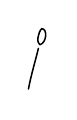
\begin{tikzpicture}[x=1pt,y=1pt,baseline=-2pt]
\draw[line width=.55pt,line cap=round] (0,-1) .. controls (1,4.3) and (2.5,9.1) .. (3.6,13.7);
\draw[line width=.55pt,line cap=round] (4.1,15) .. controls (2.8,15.8) and (3.5,19.6) .. (4.8,20.8) .. controls (7,20.9) and (6.6,15.6) .. (4.1,15);
\end{tikzpicture}}\inserted{le site}}
\normalmarginpar
\deleted{dont la catégorie sous-jacente est}\inserted{constitué par} la sous-catégorie pleine de \(S/X\) formée des objets dont le morphisme structural est dans \(\underline{M}\) , munie de la topologie induite par celle de \(S\) (III \handwritten{3}.\handwritten{1}).

1) Montrer que les familles couvrantes \((f_i:X_i\to X)_{i\varepsilon I}\) où les \(f_i\) sont dans \(\underline{M}\) forment une prétopologie sur \(S\) (II \handwritten{1}.\handwritten{3}) qui engendre la topologie de \(S\) .

2) Pour toute flèche \(u:X\to Y\) de \(S\) , montrer que le foncteur changement de base par \(u\) est un foncteur continu (III \handwritten{1}.\handwritten{1}) de \(S(Y)\) dans \(S(X)\) . \unsure{\(\mathbb{O}\)|\deleted{o}O|\deleted{O}o}n notera
\[
S(u)^{\handwritten{*}}:S(Y)^{\handwritten{\sim}}\to S(X)^{\handwritten{\sim}}
\]
le foncteur correspondant entre les catégorie\handwritten{s} de faisceaux (III \handwritten{1}.\handwritten{2},iv)).

3) Définir une équivalence entre le topos \(S^{\handwritten{\sim}}\) et la catégorie des systèmes
\[
(F_X)\ (X\varepsilon\operatorname{ob}S)\quad,\quad(\handwritten{\varphi_u})\ (u\varepsilon\mathrm{Fl}\ S)
\]
formés d'objets \(F_X\varepsilon\operatorname{ob}S(X)^{\handwritten{\sim}}\) , et pour toute flèche \(u:X\to Y\) dans \(S\) , d'un morphisme \(\handwritten{\varphi}_u:S(u)^{\handwritten{*}}(F_Y)\to F_X\) , ces systèmes
% archive sheet number: 9
